\documentclass{beamer}
\usepackage{graphicx}
\usepackage[utf8]{inputenc}
\usepackage[T1]{fontenc}
\usepackage{tikz}
\usepackage{circuitikz}
\usetheme{default}

\title{Izrada elektricnih dijagrama}
\subtitle{LaTeX}

\author{~Berto Lušetić \and ~Ivan Svoboda \and ~Dario Ćirić}

\institute[Sveučilište u Rijeci TEHNIČKI FAKULTET] 

\begin{document}

\begin{frame}
  \titlepage
\end{frame}

\begin{frame}{Outline}
  \tableofcontents
\end{frame}

\section{Što je Circuitikz?}

\begin{frame}{Što je Circuitikz}
  \begin{itemize}
    \item {Circuitikz je paket koji nam omogućuje laganu izradu električnih dijagrama u LaTex-u}
    \item {}
    \begin{figure}
      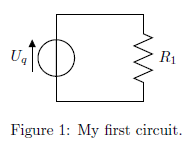
\includegraphics
      {/slike/slika1.png}
    \end{figure}
  \end{itemize}
\end{frame}

\section{Kako koristiti Circuitikz paket?}


\begin{frame}{Kako koristiti Circuitikz paket?}
  \begin{itemize}
  \item {
    Za dodavanje dijagrama trebamo koristiti paket 
    include{circuitikz}
  }
  \item{
    Svi elementi dijagrama nalazit će se unutar figure
  }
  \item{
  Naredbom begin{circutikz} započinjemo okruženje dijagrama
  }
  \end{itemize}
\end{frame}

\begin{frame}
    \begin{center}
        \begin{circuitikz}
          \draw (0,0)
          to[V,v=$U_q$] (0,2) % The voltage source
          to[short] (2,2)
          to[R=$R_1$] (2,0) % The resistor
          to[short] (0,0);
        \end{circuitikz}
    \end{center}
    \begin{center}
        \begin{figure}
          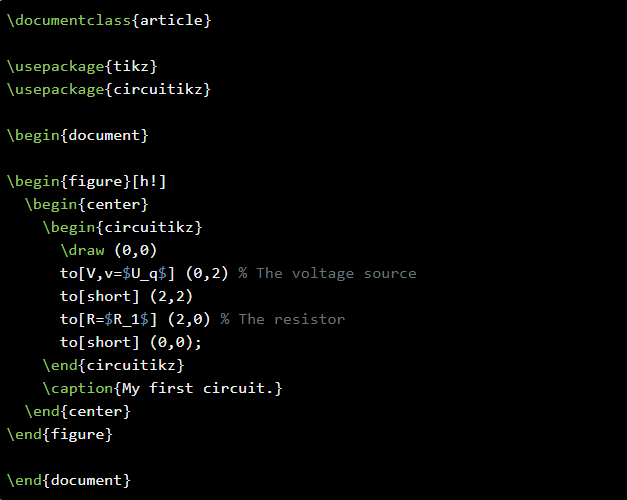
\includegraphics
          {/slike/slika2.png}
        \end{figure}
    \end{center}
\end{frame}

\section{Kada i zašto koristiti Circuitikz paket?}

\begin{frame}{Zašto koristiti Circuitikz paket?}
  \begin{itemize}
  \item {
    Korištenje paketa Circuitikz često je najbolji i
    najpregledniji način crtanja električnih krugova
    ili sklopova
  }
  \item{
    S dobrom dokumentacijom i jednostavnošću načina korištenja
    svakako je jedan od prvih izbora za izradu takvih 
    dokumenata.
  }
  \end{itemize}
\end{frame}

\begin{frame}{Kada koristiti Circuitikz paket?}
  \begin{itemize}
  \item {
    Circuitikz paket koristi se u izradi diplomskih i doktorskih
    radova, te općenito u radu sa ili prezentiranju strujnih
    krugova
  }
  \item{
    Široki spektar mogućnosti i broj elemenata strujnih krugova
    osigurava mogućnost rada i zahtjevnim korisnicima
  }
  \begin{figure}
      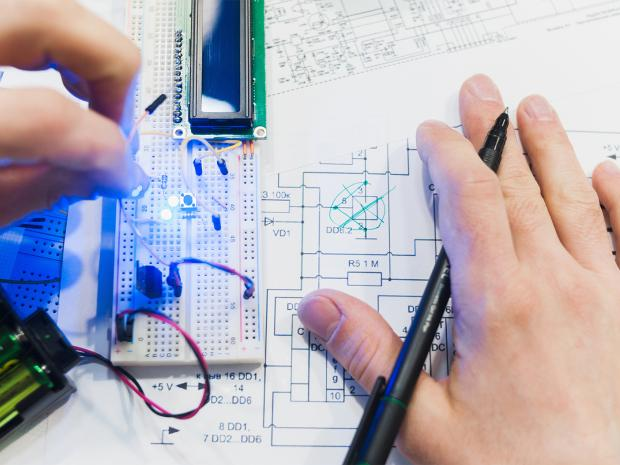
\includegraphics
      {/slike/slika3.jpg}
    \end{figure}
  \end{itemize}
\end{frame}

\begin{frame}
  \begin{itemize}
  \item {
    First item.
  }
  \item {   
    Second item.
  }

  \item<3-> {
    Third item.
  }
  \item<4-> {
    Fourth item.
  }
  
  \item<5-> {
    Fifth item. \uncover<6->{Extra text in the fifth item.}
  }
  \end{itemize}
\end{frame}

\section{Second Main Section}

\subsection{Another Subsection}

\appendix
\section<presentation>*{\appendixname}
\subsection<presentation>*{For Further Reading}

\begin{frame}[allowframebreaks]
  \frametitle<presentation>{For Further Reading}
    
  \begin{thebibliography}{10}
    
  \beamertemplatebookbibitems
  % Start with overview books.

  \bibitem{Author1990}
    A.~Author.
    \newblock {\em Handbook of Everything}.
    \newblock Some Press, 1990.
 
    
  \beamertemplatearticlebibitems
  % Followed by interesting articles. Keep the list short. 

  \bibitem{Someone2000}
    S.~Someone.
    \newblock On this and that.
    \newblock {\em Journal of This and That}, 2(1):50--100,
    2000.
  \end{thebibliography}
\end{frame}

\end{document}


